% !TeX spellcheck = pt_BR
\documentclass[aspectratio=169, xcolor=dvipsnames]{beamer} 
%Definições de tema
\setbeamertemplate{blocks}[rounded][shadow=false]
\usetheme{Madrid}
\setbeamertemplate{items}[square]
\setbeamertemplate{caption}[numbered]
\usecolortheme{beaver}
\setbeamercolor{frametitle}{bg=white!10!white}

\usefonttheme{professionalfonts} 
\setbeamertemplate{itemize item}{\color[rgb]{0.8,0,0}$\blacksquare$}
\setbeamertemplate{itemize subitem}{\color[rgb]{0.8,0,0}$\blacksquare$}
\setbeamertemplate{itemize subsubitem}{\color[rgb]{0.8,0,0}$\blacksquare$}

%Definições de seção
\setcounter{secnumdepth}{3}
\setcounter{tocdepth}{2}


\usepackage{xkeyval}
\usepackage{todonotes}
\presetkeys{todonotes}{inline}{}


\usepackage{helvet}
\renewcommand{\familydefault}{\sfdefault}
\usepackage{float}
\usepackage[brazil]{babel}
\usepackage[utf8]{inputenc}
\usepackage{graphicx, tikz}
\usepackage{url}
\usepackage{subfigure}
\usepackage{mathtools} % setas com texto
\usepackage{multicol}
\usepackage{listings}
\usepackage{lipsum}
\usepackage{scalefnt}
\usepackage{ragged2e}
\usepackage{etoolbox, verbatim}

% Listing
\lstset{ 
	numbers=left,
	stepnumber=1,
	numbersep=6pt,
	numberstyle=\small\color{black},
	basicstyle= \scriptsize,
%	keywordstyle=\color{black},
%	commentstyle=\color{black},
%	stringstyle=\color{black},
	tabsize=2
}
%Definições Listing - Linguagem Scala
\lstdefinelanguage{scala}{
morekeywords={abstract,case,catch,class,def,%
	do,else,extends,false,final,finally,%
	for,if,implicit,import,match,mixin,%
	new,null,object,override,package,%
	private,protected,requires,return,sealed,%
	super,this,throw,trait,true,try,%
	type,val,var,while,with,yield},
otherkeywords={=>,<-,<\%,<:,>:,\#,@},
sensitive=true,
morecomment=[l]{//},
morecomment=[n]{/*}{*/},
morestring=[b]",
morestring=[b]',
morestring=[b]"""
}

\let\olditem=\item% 
\renewcommand{\item}{\olditem \justifying}

\title[Processamento Digital de Imagem - \textit{Face Detection}]{\textbf{Processamento Digital de Imagem}\\\textit{Face Detection - Referencial Teórico}}
\author[rodolfolabiapari@decom.ufop.br]{Rodolfo Labiapari Mansur Guimarães}
\institute[IFMG]{\begin{figure}
			\centering
			
\includegraphics[width=0.1\textwidth]{img/ufop.jpg}
		\end{figure}}
\institute[UFOP]{
	\textit{rodolfolabiapari@decom.ufop.br} \\
	Lattes: \url{http://goo.gl/MZv4Dc} \\
	Departamento de Computação -- Universidade Federal de Ouro Preto \\
	Ouro Preto - MG -- Brasil }

\date[\today]{Última Atualização: \today.}

\begin{document}


\frame{\titlepage}

\AtBeginSection[] 
{
	\begin{frame}
	\frametitle{Sumário}
	\tableofcontents[]
	\end{frame}
}

\AtBeginSubsection[] 
{
	\begin{frame}
	\frametitle{Sumário}
	\tableofcontents[
    currentsection, 
    currentsubsection, 
    hideothersubsections, 
    %sectionstyle=show/hiden, 
    subsectionstyle=show/shaded, ]
	\end{frame}
}

%\usebackgroundtemplate{
\includegraphics[trim=0cm 0cm 10cm 0cm, width=0.03\textwidth]{img/ufop.jpg}}

\section{Estudo Bibliográfico}
\begin{frame}{Introdução}
	\begin{itemize}
		\setlength{\itemsep}{1.5em}
		\item \textit{Face detection}  é uma tecnologia de computadores usada em várias aplicações para identificação de faces humanas em imagens digitais, o que justifica a vasta necessidade de pesquisa nesta área.
		
		\item Todos os métodos analisados aqui são para imagens em escala de cinza.
	\end{itemize}
\end{frame}


\begin{figure}
	\centering
	\label{fig:inst}
	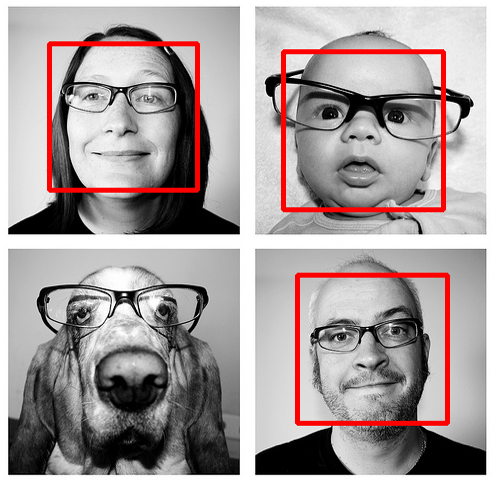
\includegraphics[width=0.48\textwidth]{img/intro1.png}
	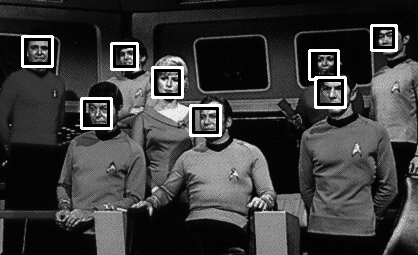
\includegraphics[width=0.48\textwidth]{img/intro2.jpg}
\end{figure}

\section{Surveys}
\begin{frame}{Surveys}
	\begin{itemize}
		\setlength{\itemsep}{1.5em}
		\item Zhang, em \textit{A survey of recent advances in face detection} \cite{zhang2010survey}, e Hjelmaas, \textit{Face Detection: A Survey} \cite{hjelmaas2001face}, realizaram um estudo qualificativo para as várias abordagens existente. 
		
		\item Explicam que o tema possui várias categorias sendo estas o Processamento em:
		\begin{enumerate}
			\setlength{\itemsep}{1em}
			\item Vídeo ou;
			\item Imagem e subníveis mais baixos como cor, posição, rotação, oclusão e muitas outras focos de pesquisa. 
		\end{enumerate}
	\end{itemize}
\end{frame}

\section{O Pioneiro}
\begin{frame}{O Pioneiro}
	\begin{itemize}
		\setlength{\itemsep}{1.5em}
		\item Sakai \cite{sakai1972computer} foi um dos primeiros a pesquisar algoritmos. 
		
		\item Na suas pesquisas, as instâncias deveriam ser simplistas e padronizadas
		\begin{itemize}
			\item A face posta de forma frontal, sem obstrução de elementos do rosto e sem fundos complexos na imagem.
			\item Qualquer variação deste cenário resultaria numa execução sem resultados confiantes.
		\end{itemize}
		
		\item Seu algoritmo se baseia de uma árvore de decisão onde verifica, da forma mais geral pra mais específica, se o quadro que está analisando é formado por elementos de um rosto humano. 
		\begin{itemize}
			\item Assim, a cada nível avançado, mais certo é de ser um rosto humano
		\end{itemize}
		
		\item Quando acontece alguma negação de determinado nível, realiza-se outras tentativas consecutivas a fim de identificar se realmente o item é uma face.
		\begin{itemize}
			\item Realizando outros testes consecutivos permite-se identificar se a face está em alguma posição diferente do modo perfil frontal esperado.
		\end{itemize}
	\end{itemize}
\end{frame}

\begin{figure}
	\centering
	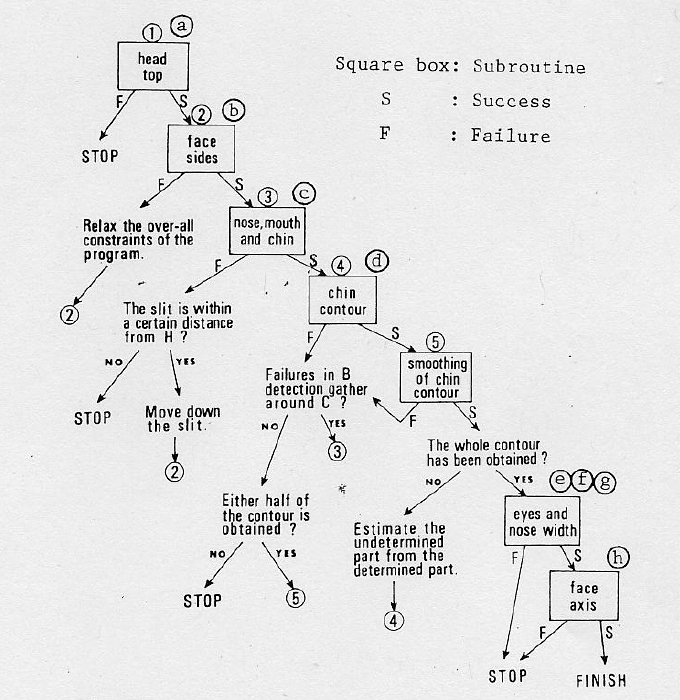
\includegraphics[width=0.54\textwidth]{img/sakai.png}
\end{figure}

\section{Categorização do Problema}
\begin{frame}{Categorização do Problema}
	\begin{itemize}
		\setlength{\itemsep}{1.5em}
		\item Atualmente, existe vários métodos de detecção/localização de faces em imagens em escala de cinza. 
		
		\item Os métodos atuais são baseados em:
		
		\begin{itemize}
			\setlength{\itemsep}{0.8em}
			\item Conhecimento;
			\item Características Invariantes;
			\item Casamento de Formatos;
			\item e Aparência.
		\end{itemize}
		
	\end{itemize}
\end{frame}

\subsection{Métodos baseado em Conhecimento}
\begin{frame}{Métodos baseado em Conhecimento}
	\begin{itemize}
		\setlength{\itemsep}{1.5em}
		\item Utilizam abordagem \textit{top-down} e são classificados como métodos simples e restritos. 
		
		\item Yang \cite{yang1994human} desenvolveu pesquisas onde é realizado processos de alteração da resolução a procura de pontos interessantes da figura 
		\begin{itemize}
			\setlength{\itemsep}{1em}
			\item Após localizado determinado ponto de interesse, é feito o histograma dos pontos da imagem a procura de padrões conhecidos como de olhos, nariz e boca de acordo com a tonalidade da imagem.
			
			\item Já sabe-se pela literatura que olhos, nariz, orelhas e boca possuem tonalidade diferente da pele do rosto como um todo.
		\end{itemize}
	\end{itemize}
\end{frame}

\begin{frame}{Métodos baseado em Conhecimento}
	\begin{figure}
		\centering
		\label{fig:inst}
		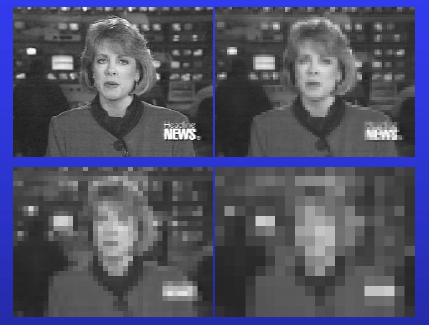
\includegraphics[width=0.6\textwidth]{img/m1-1.png}
	\end{figure}
\end{frame}

\begin{frame}{Métodos baseado em Conhecimento}
	\begin{figure}
		\centering
		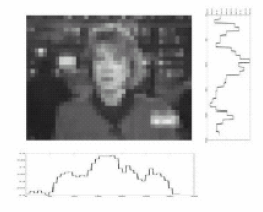
\includegraphics[width=0.6\textwidth]{img/m1-3.png}
	\end{figure}
\end{frame}

\begin{frame}{Métodos baseado em Conhecimento}
	\begin{figure}
		\centering
		\label{fig:inst}
		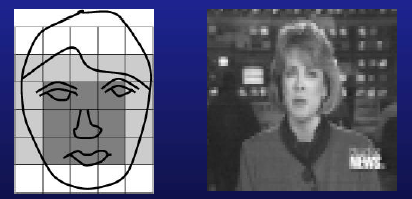
\includegraphics[width=0.6\textwidth]{img/m1-2.png}
	\end{figure}
\end{frame}

\subsection{Abordagem em Características Invariantes}
\begin{frame}{Abordagem em Características Invariantes}
	\begin{itemize}
		\setlength{\itemsep}{1.5em}
		\item Procura encontrar relações padronizadas como olhos, nariz, boca, orelhas, textura, etc. 
		
		\item Yow \cite{yow1996probabilistic} \cite{yow1997feature} utiliza filtros para encontrar regiões relevantes e, em seguida, tentar encontrar formas conhecidas de faces e identificá-la na foto.
		
	\end{itemize}
\end{frame}

\begin{frame}
	\begin{figure}
		\centering
		\label{fig:inst}
		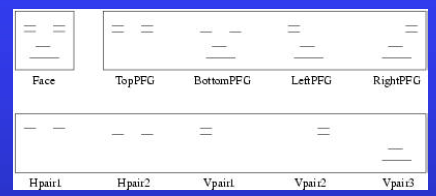
\includegraphics[width=0.6\textwidth]{img/m4-1.png}\\\pause
		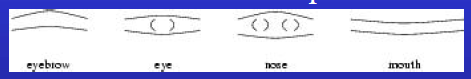
\includegraphics[width=0.6\textwidth]{img/m4-2.png}\\\pause
		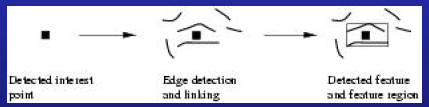
\includegraphics[width=0.6\textwidth]{img/m4-3.png}
	\end{figure}
\end{frame}

\subsection{Métodos de Casamento de Template}
\begin{frame}{Métodos de Casamento de Template}
	\begin{itemize}
		\setlength{\itemsep}{1.5em}
		\item É um método que utiliza máscaras que tentam realizar combinações do quadro analisado com o modelo de resposta requisitada. 
		
		\item Selecionado um quadro, é feito comparações com a luminosidade do local avaliado visando sempre o modelo e ao final classificando se este ponto interessante é de fato uma face. 
		\begin{itemize}
			\setlength{\itemsep}{1em}
			\item Abordagem simples;
			\item Mas requer que o algoritmo tenha modelos pré-definidos/treinados o que dificulta a diversidade do mundo real de dados e situações.
		\end{itemize}
	\end{itemize}
\end{frame}

\begin{frame}{Métodos de Casamento de Template}
	\begin{figure}
		\centering
		\label{fig:inst}
		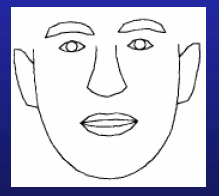
\includegraphics[width=0.32\textwidth]{img/m2-1.png}\pause
		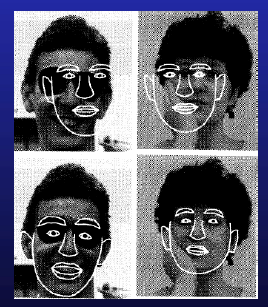
\includegraphics[width=0.32\textwidth]{img/m2-2.png}\pause
		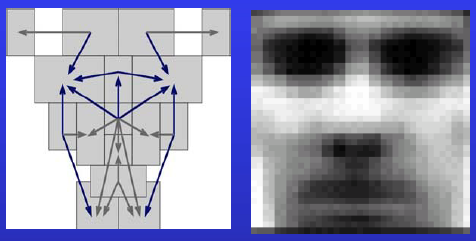
\includegraphics[width=0.32\textwidth]{img/m2-3.png}
	\end{figure}
\end{frame}

\subsection{Aparência}
\begin{frame}{Aparência}
	\begin{itemize}
		\item Geralmente utiliza-se de Rede Neurais como o Perceptron de múltiplas camadas, e outros procedimentos para categorizar uma face.
	\end{itemize}
\end{frame}

\begin{frame}{Aparência}
\begin{figure}
	\centering
	\label{fig:inst}
	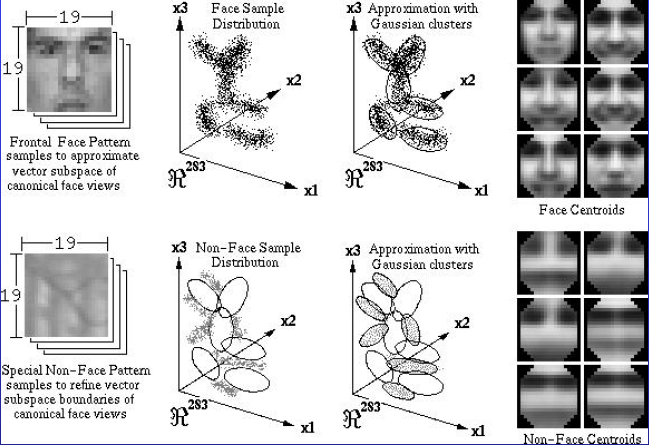
\includegraphics[width=0.7\textwidth]{img/m3-1.png}
\end{figure}
\end{frame}

\frame{\titlepage}

\bibliographystyle{sbc}
\bibliography{sbc-template}

\frame{\titlepage}


\end{document}